\section{EC 2.7}

\textbf{Exercise 7.0.1} (Maxmin strategy definition). \textit{Provide the definition of Maxmin strategy in 2–player normal–form games.}\\\\
The problem of finding a Maxmin strategy of player $i$ against
player $-i$ is formulated as:
\begin{align*}
\arg \max _{\sigma_{i}}  & \quad \min_{\sigma_{-i}} & \sum_{a_{i} \in A_{i}} \sum_{a_{-i} \in A_{-i}}\left[U_{i}\left(a_{i}, a_{-i}\right) \sigma_{i}\left(a_{i}\right) \sigma_{-i}\left(a_{-i}\right)\right] & &\\
& \quad s.t. & \sum_{a_{-i} \in A_{-i}} \sigma_{-i}\left(a_{-i}\right) & =1\\
& & \sigma_{-i}\left(a_{-i}\right) & \geqslant 0 & \forall a_{-i} \in A_{-i}\\
s.t. & \sum_{a_{i} \in A_{i}} \sigma_{i}\left(a_{i}\right) & & =1\\
& \sigma_{i}\left(a_{i}\right) & & \geqslant 0 & \forall a_{i} \in A_{i}\\
\end{align*}
\textbf{Exercise 7.0.2} (Maxmin strategy example). \textit{Given a 2–player normal–form games with 2 actions per player, find a Maxmin strategy.}\\\\
Consider the following 2-player matrix game in which player 1 plays as max player and player 2 plays as min player:
\begin{figure}[H]
\centering
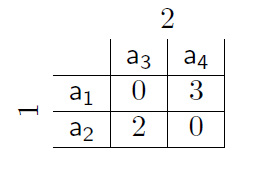
\includegraphics[scale=0.6]{images/img_2_7_01.png}
\end{figure}
\noindent
We report the strategy simplex of player 1 partitioned in subareas with the corresponding action player 2 would play and subsequently how the expected utility of player 1 varies in the simplex given the strategy of player 2. The Maxmin value of player 1 is 1.2.
\begin{figure}[H]
\centering
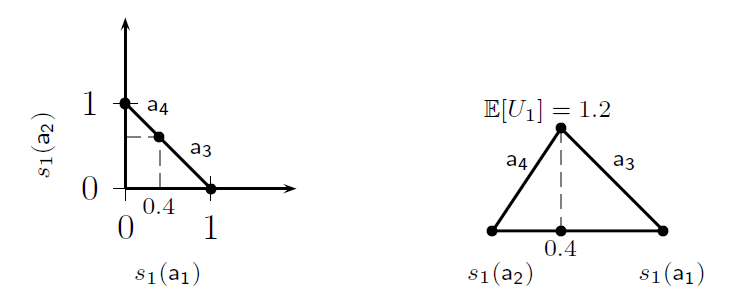
\includegraphics[scale=0.6]{images/img_2_7_02.png}
\end{figure}
\noindent
\textbf{Exercise 7.0.3} (Complexity). \textit{What is the computational complexity of finding the Maxmin/Minmax strategy with 2–player normal–form games?}\\\\
The Maxmin strategy and the corresponding Maxmin value of player $i$ against player $-i$ can be found in polynomial time in the size of the game, where the size is given by the number of actions of the players. Therefore the Maxmin finding problem is in \textsf{FP} class.\\\\
\textbf{Exercise 7.0.4} (Mathematical programming formulation). \textit{Given a 2–player normal–form game, provide the mathematical programming formulation for finding a Maxmin/Minmax strategy and show its derivation.}\\\\
The Maxmin strategy and the corresponding value of player $ i $
against player $ -i $ can be found by solving the following Linear Program (LP):
$$
\begin{aligned}
\arg \max_{\sigma_{i}, v_j} & \quad v_{i} \\
\text{s.t.} & \quad v_{i}-\sum_{a_{i} \in A_{i}}\left[U_{i}\left(a_{i}, a_{-i}\right) \sigma_{i}\left(a_{i}\right)\right] & \quad \leqslant 0 & \quad \forall a_{-i} \in A_{-i} \\
& \sum_{a_{i} \in A_{i}} \sigma_{i}\left(a_{i}\right) & \quad =1 &\\
& \sigma_{i}\left(a_{i}\right) & \quad \geqslant  0 & \quad \forall a_{i} \in A_{i}
\end{aligned}
$$
\begin{figure}[H]
\centering
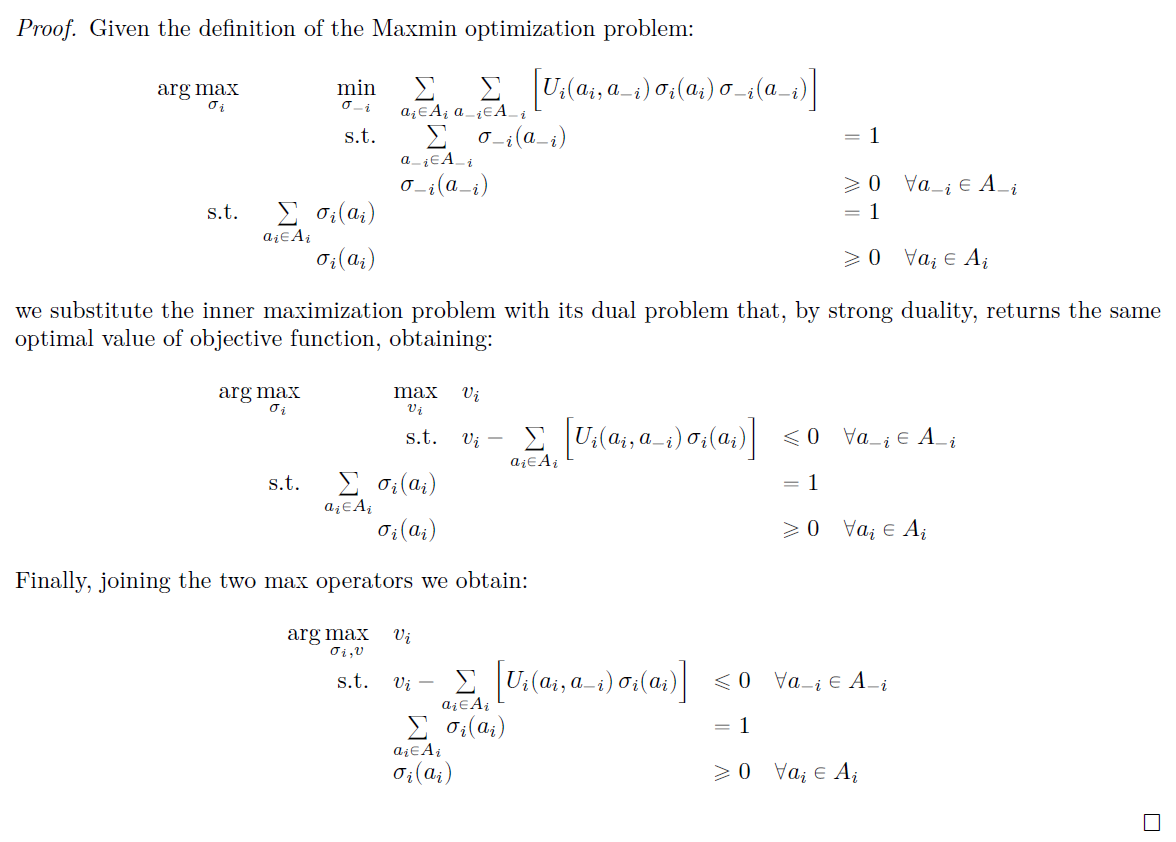
\includegraphics[width=\textwidth]{images/img_2_7_03.png}
\end{figure}
%Proof. Given the definition of the Maxmin optimization problem:
%$$
%\begin{aligned}
%\arg \max _{\sigma_{i}} \quad  & \min & _{\sigma_{-i}} \sum_{a_{i} \in A_{i}} \sum_{a_{-i} \in A_{-i}}\left[U_{i}\left(a_{i}, a_{-i}\right) \sigma_{i}\left(a_{i}\right) \sigma_{-i}\left(a_{-i}\right)\right] & &\\
%& s.t. & \sum_{a_{-i} \in A_{-i}} \sigma_{-i}\left(a_{-i}\right) & =1\\
%& & \sigma_{-i}\left(a_{-i}\right) & \geqslant 0 & \forall a_{-i} \in A_{-i}\\
%s.t. & \sum_{a_{i} \in A_{i}} \sigma_{i}\left(a_{i}\right) & & =1\\
%& \sigma_{i}\left(a_{i}\right) & & \geqslant 0 & \forall a_{i} \in A_{i}\\
%\end{aligned}
%$$
%we substitute the inner maximization problem with its dual problem that, by strong duality, returns the same optimal value of objective function, obtaining
%$$
%\begin{aligned}
%\arg \max_{\sigma_{i}, v_j} & \quad v_{i} \\
%\text{s.t.} & \quad v_{i}-\sum_{a_{i} \in A_{i}}\left[U_{i}\left(a_{i}, a_{-i}\right) \sigma_{i}\left(a_{i}\right)\right] & \quad \leqslant 0 & \quad \forall a_{-i} \in A_{-i} \\
%& \sum_{a_{i} \in A_{i}} \sigma_{i}\left(a_{i}\right) & \quad =1 &\\
%& \sigma_{i}\left(a_{i}\right) & \quad \geqslant  0 & \quad \forall a_{i} \in A_{i}
%\end{aligned}
%$$
%Finally, joining the two max operators we obtain:
%$$
%\begin{aligned}
%\arg \max_{\sigma_{i}, v_j} & \quad v_{i} \\
%\text{s.t.} & \quad v_{i}-\sum_{a_{i} \in A_{i}}\left[U_{i}\left(a_{i}, a_{-i}\right) \sigma_{i}\left(a_{i}\right)\right] & \quad \leqslant 0 & \quad \forall a_{-i} \in A_{-i} \\
%& \sum_{a_{i} \in A_{i}} \sigma_{i}\left(a_{i}\right) & \quad =1 &\\
%& \sigma_{i}\left(a_{i}\right) & \quad \geqslant  0 & \quad \forall a_{i} \in A_{i}
%\end{aligned}
%$$
\noindent
The Minmax strategy player $i$ against player $-i$ and the corresponding value of player $-i$ can be found by solving the following Linear Program:
\begin{align*}
\arg \min_{\sigma_{i}, v_j} & \quad v_{-i}\\
\text{s.t.} & \quad v_{-i}-\sum_{a_{i} \in A_{i}}\left[U_{-i}\left(a_{i}, a_{-i}\right) \sigma_{i}\left(a_{i}\right)\right] & \geqslant 0 & \quad \forall a_{-i} \in A_{-i} \\
& \sum_{a_{i} \in A_{i}} \sigma_{i}\left(a_{i}\right) & \quad =1 &\\
& \sigma_{i}\left(a_{i}\right) & \quad \geqslant  0 & \quad \forall a_{i} \in A_{i}
\end{align*}
\begin{figure}[H]
\centering
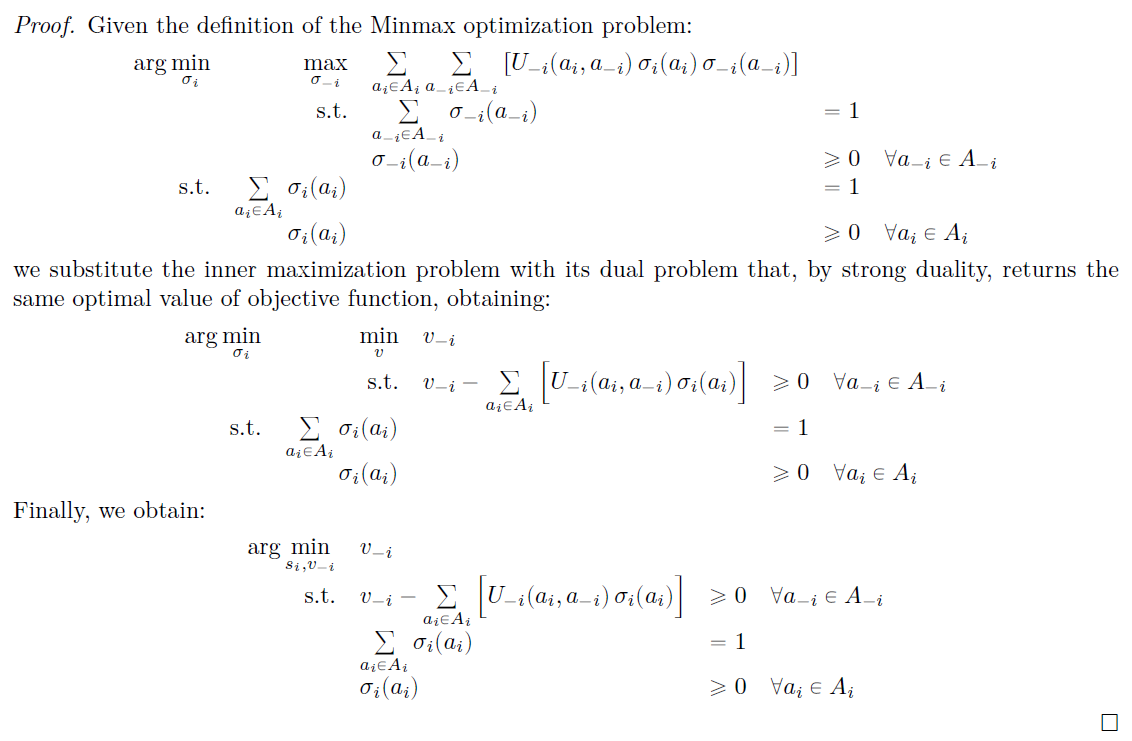
\includegraphics[width=\textwidth]{images/img_2_7_04.png}
\end{figure}
\textbf{Exercise 7.0.5} (Solving a game). \textit{Given a normal–form game with 2 players, find a Maxmin strategy by means of AMPL + GUROBI.}\\\\
\textcolor{red}{TODO}\\\\

\section{EC 2.8}

\textbf{Exercise 8.0.1} (Maxmin strategy definition). \textit{Provide the definition of Maxmin strategy in 2–player sequence– form games.}\\\\
The Maxmin strategy of player i against player $-i$ in sequence form can be found by solving the following linear mathematical programming problem:
\begin{align*}
\arg \max _{r_{i}, v_{i}}  & \sum_{h_{-i} \in H_{-i} \cup\left\{\mathrm{h}_{\varnothing}\right\}} f_{-i}\left(h_{-i}\right) v_{i}\left(h_{-i}\right)\\
\text {s.t.} & \quad \sum_{h_{-i} \in H_{-i} \cup\left\{\mathrm{h}_{\varnothing}\right\}} F_{-i}\left(h_{-i}, q_{-i}\right) v_{i}\left(h_{-i}\right)-\sum_{q_{i} \in Q_{i}}\left[U_{i}\left(q_{i}, q_{-i}\right) r_{i}\left(q_{i}\right)\right] & \leqslant & \quad 0 & \forall q_{-i} \in Q_{-i}\\
& \sum_{q_{i} \in Q_{i}} F_{i}\left(h_{i}, q_{i}\right) r_{i}\left(q_{i}\right) & = & \quad f_{i} \left(h_{i}\right) & \forall h_{i} \in H_{i} \cup\left\{\mathrm{h}_{\varnothing}\right\}\\
& r_i (q_i) & \geqslant & \quad 0 & \forall q_i \in Q_i
\end{align*}
\noindent
\textbf{Exercise 8.0.2} (Complexity). \textit{What is the computational complexity of finding the Maxmin/Minmax strategy with 2–player sequence–form games?}\\\\
The Maxmin strategy and the corresponding Maxmin value of player $i$ against player $-i$ in an extensive-form game can be found, by means of the sequence-form representation, in polynomial time in the size of the game, where the size is given by the number of nodes
of the game tree. Therefore the Maxmin finding problem is in \textsf{FP} class.\\\\
\textbf{Exercise 8.0.3} (Mathematical programming formulation). \textit{Given a 2–player sequence–form game, provide the mathematical programming formulation for finding a Maxmin/Minmax strategy and show its derivation.}\\\\
The Minmax strategy of player i against player $-i$ in sequence form can be found by solving the following linear mathematical programming problem:
\begin{align*}
\arg \min _{r_{i}, v_{-i}}  & \sum_{h_{-i} \in H_{-i} \cup\left\{\mathrm{h}_{\varnothing}\right\}} f_{-i}\left(h_{-i}\right) v_{i}\left(h_{-i}\right)\\
\text {s.t.} & \quad \sum_{h_{-i} \in H_{-i} \cup\left\{\mathrm{h}_{\varnothing}\right\}} F_{-i}\left(h_{-i}, q_{-i}\right) v_{i}\left(h_{-i}\right)-\sum_{q_{i} \in Q_{i}}\left[U_{-i}\left(q_{i}, q_{-i}\right) r_{i}\left(q_{i}\right)\right] & \leqslant & \quad 0 & \forall q_{-i} \in Q_{-i}\\
& \sum_{q_{i} \in Q_{i}} F_{i}\left(h_{i}, q_{i}\right) r_{i}\left(q_{i}\right) & = & \quad f_{i} \left(h_{i}\right) & \forall h_{i} \in H_{i} \cup\left\{\mathrm{h}_{\varnothing}\right\}\\
& r_i (q_i) & \geqslant & \quad 0 & \forall q_i \in Q_i
\end{align*}
\noindent
\textbf{Exercise 8.0.4} (Solving a game). \textit{Given a sequence–form game with 2 players, find a Maxmin strategy by means of AMPL + GUROBI.}\\\\
\textcolor{red}{TODO}\\\\

\section{EC 2.9}

\textbf{Exercise 9.0.1} (Team Maxmin strategy definition). \textit{Provide the definition of the Maxmin strategy when there are multiple max players and a single min player.}\\\\
\textbf{Many-max player/single-min players.} Now, we focus on the case in which there are multiple max players and only one min player. Initially, we remark that this situation makes sense only when the utility functions of all the max players are the same, otherwise it would not be clear which objective function the max players should maximize. Therefore, in this case, the max players are forming a team and searching for the Maxmin strategy is equivalent to searching for a Team-Maxmin strategy. Also here, we can distinguish the case in which the team plays in correlated strategies from the case in which the team plays in mixed strategies. We initially focus on the first case.\\\\
(Maxmin optimization problem (with correlated min players)). The problem of finding a Maxmin strategy of a team of $n-1$ players, playing in correlated fashion, against player $i$ is formulated as:
\begin{align*}
\arg \max _{\bm{\sigma}_{-i}}  & \quad \min_{\sigma_{i}} & \sum_{\mathbf{a}_{-i} \in A_{-i}} \sum_{a_{i} \in A_{i}}\left[U_{-i}\left(a_{i}, \mathbf{a}_{-i}\right) \sigma_{i}\left(a_{i}\right) \bm{\sigma}_{-i}\left(\mathbf{a}_{-i}\right)\right] & &\\
& \quad s.t. & \sum_{a_{i} \in A_{i}} \sigma_{i}\left(a_{i}\right) & =1\\
& & \sigma_{i}\left(a_{i}\right) & \geqslant 0 & \forall a_{i} \in A_{i}\\
s.t. & \sum_{\mathbf{a}_{-i} \in A_{-i}} \bm{\sigma}_{i}\left(\mathbf{a}_{-i}\right) & & =1\\
& \bm{\sigma}_{i}\left(\mathbf{a}_{-i}\right) & & \geqslant 0 & \forall \mathbf{a}_{-i} \in A_{-i}\\
\end{align*}
\noindent
(Maxmin optimization problem (with non-correlated min players)). The problem of finding a
Maxmin strategy of a team of $n-1$ players, playing in mixed strategies, against player $i$ is formulated as:
\begin{align*}
\arg \max _{\bm{\sigma}_{-i}}  & \quad \min_{\sigma_{i}} & \sum_{a_{i} \in A_{i}} \sum_{\mathbf{a}_{-i} \in A_{-i}} \left[U_{-i}\left(a_{i}, \mathbf{a}_{-i}\right) \prod_{j \in N}{\sigma_j (a_j)} \right] & &\\
& \quad s.t. & \sum_{a_{i} \in A_{i}} \sigma_{i}\left(a_{i}\right) & =1\\
& & \sigma_{i}\left(a_{i}\right) & \geqslant 0 & \forall a_{i} \in A_{i}\\
s.t. & \sum_{a_{j} \in A_{j}} \sigma_{i}\left(a_{j}\right) & & =1 & \forall j \in N \setminus \{i\} \\
& \sigma_{j}\left(a_{j}\right) & & \geqslant 0 & \forall j \in N \setminus \{i\}, \forall a_{j} \in A_{j}\\
\end{align*}
\noindent
\textbf{Exercise 9.0.2} (Complexity). \textit{What is the computational complexity of finding the Maxmin strategy with n–max players and 1 min player in normal–form games (equivalently finding a Minmax strategy with n–min player and 1 max player)?}\\\\
The Maxmin strategy and the corresponding Maxmin value of $n$ min-players against 1 max-player can be found in polynomial time in the size of the game, where the size is given by the number of actions of the players. Therefore the Maxmin finding problem is in \textsf{FP} class.\\\\
\textbf{Exercise 9.0.3} (Mathematical programming formulation). \textit{Given an n–player normal–form game, provide the mathematical programming formulation for finding a Maxmin strategy and show its derivation when there are $ n-1 $ max players and $ 1 $ min players.}\\\\
(Maxmin strategy formulation (with correlated min players)). The Maxmin strategy and the corresponding value of a team of $n-1$ players, playing in correlated fashion, against player i can be found by solving the following Linear Program:
\begin{figure}[H]
\centering
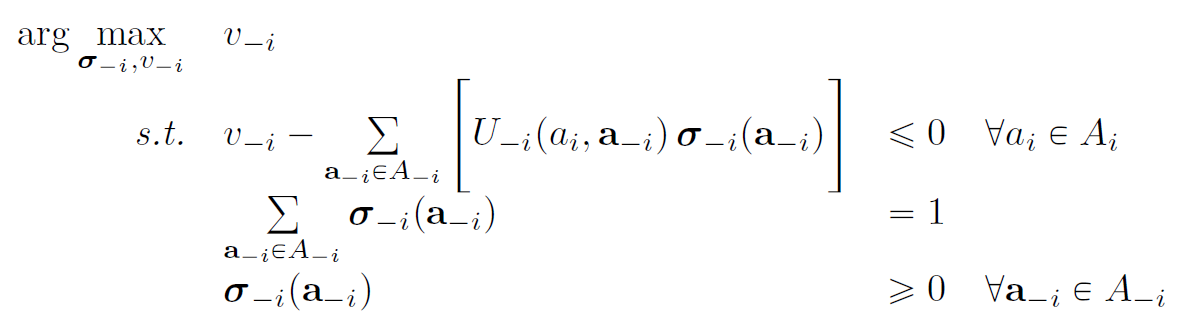
\includegraphics[width=\textwidth]{images/img_2_9_03.png}
\end{figure}
\noindent
\textbf{Exercise 9.0.4} (Solving a game). \textit{Given a normal–form game with n players among which $ n-1 $ are maximizers and $ 1 $ is a minimizer, find a Maxmin strategy by means of AMPL + BARON.}\\\\
\textbf{Exercise 9.0.5} (L’ho aggiunta io). \textit{Provide the definition and the mathematical programming formulation of the Maxmin strategy when there is a single max player and multiple min players.}\\\\
(Maxmin optimization problem (with correlated min players)). The problem of finding a Maxmin strategy of player i against $n-1$ players, playing in correlated fashion, is formulated as:
\begin{figure}[H]
\centering
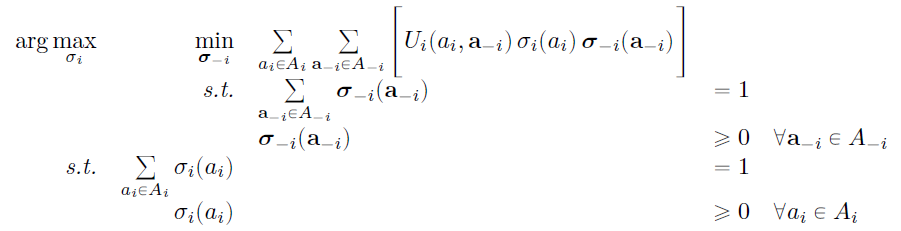
\includegraphics[width=\textwidth]{images/img_2_9_04.png}
\end{figure}
\noindent
We can easily derive the mathematical program solving the above problem.\\
(Maxmin strategy formulation (with correlated min players)). The Maxmin strategy and the corresponding value of player i against $n-1$ correlated players can be found by solving the following Linear Program:
\begin{figure}[H]
\centering
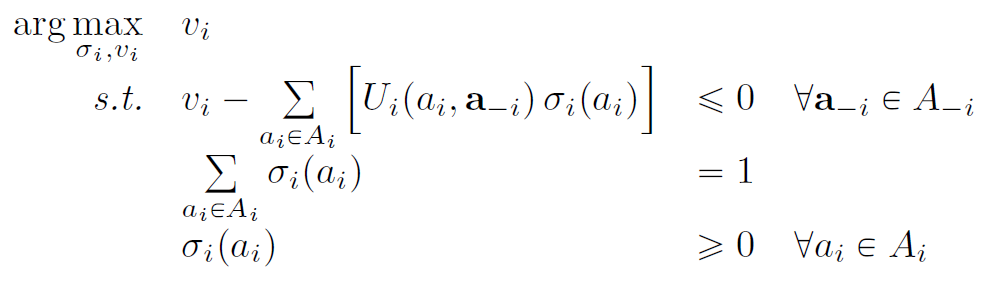
\includegraphics[width=\textwidth]{images/img_2_9_05.png}
\end{figure}
\noindent
(Maxmin strategy formulation (with correlated min players)). The problem of finding a Maxmin strategy with multiple min players playing correlated strategies is equivalent to the problem of finding a Maxmin strategy with a single min players, in which the actions available to this player are all the possible joint actions of all the min players.\\
Let us consider the case in which the min players play mixed strategies and therefore they cannot correlate.\\
(Maxmin optimization problem (with non-correlated min players)). The problem of finding a Maxmin strategy of player i against $n-1$ players, each playing independently from the others, is formulated
as:
\begin{figure}[H]
\centering
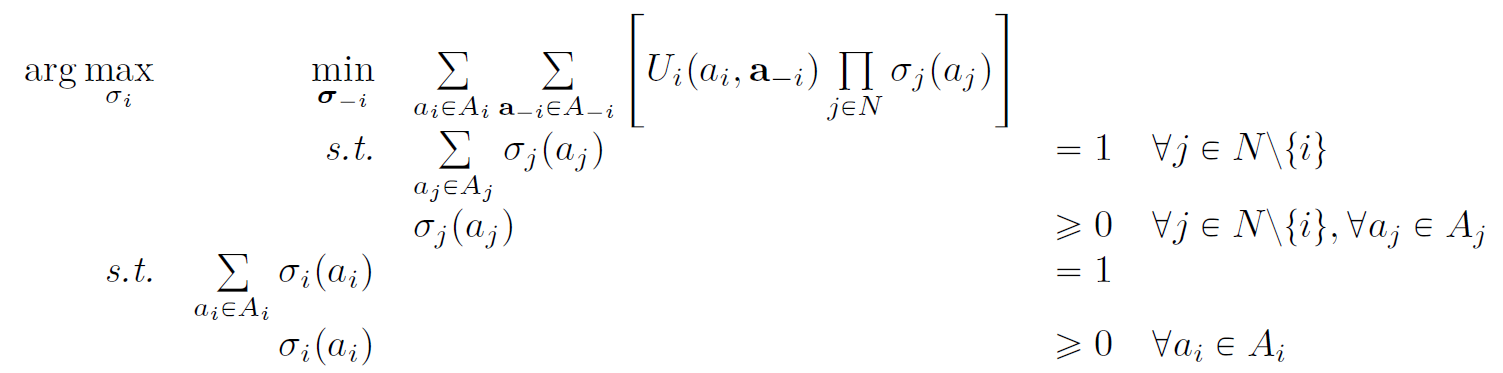
\includegraphics[width=\textwidth]{images/img_2_9_06.png}
\end{figure}
\noindent
In this case, the problem of deriving a finite (in terms of variables and constraints) mathematical program
is open. The crucial issue concerns the impossibility to reformulate the minimization problem since it is not
linear and therefore strong duality cannot be applied.
\section{EC 2.10}

\textbf{Exercise 10.0.1} (Sperner’s labeling). \textit{Provide the definition of Sperner’s labeling.}\\\\
(Simplicial subdivision). A simplicial subdivision of an n-dimensional simplex $\Delta^n$ is a finite set of subsimplices $\mathcal{D} = \{\Delta_i^n\}$ for which $\bigcup_{\Delta_i^n \in \mathcal{D}}{\Delta_i^n} = \Delta^n$, and for any $\Delta_i^n, \Delta_j^n \in \mathcal{D}$ the set $\Delta_i^n \cap \Delta_j^n$ is either empty or equal to a common facet.\\
(Sperner’s labeling). Given a n-dimensional simplex and a simplicial subdivion $ \mathcal{D} $, a Sperner’s labeling is a labeling of the vertices V of the subsimplices with labels $L = \{ 0, 1, \ldots, n \}$ is a function $l : V \rightarrow L$
satisfying the following conditions:
\begin{itemize}
\item each one of the $n+1$ vertices of the simplex is labeled with a label different from the label of the others;
\item the vertices of a subsimplex that lie on the facet of the simplex whose vertices have labels in $\{ 1, \ldots , n \}$ have label in $\{ 1, \ldots , n \}$ (a similar condition holds for the vertices on the other facets);
\item there is no restriction on the labeling of the vertices in the interior of the simplex.
\end{itemize}
An example of Sperner’s labeling of the above simplex $\Delta^2$ is as follows:
\begin{figure}[H]
\centering
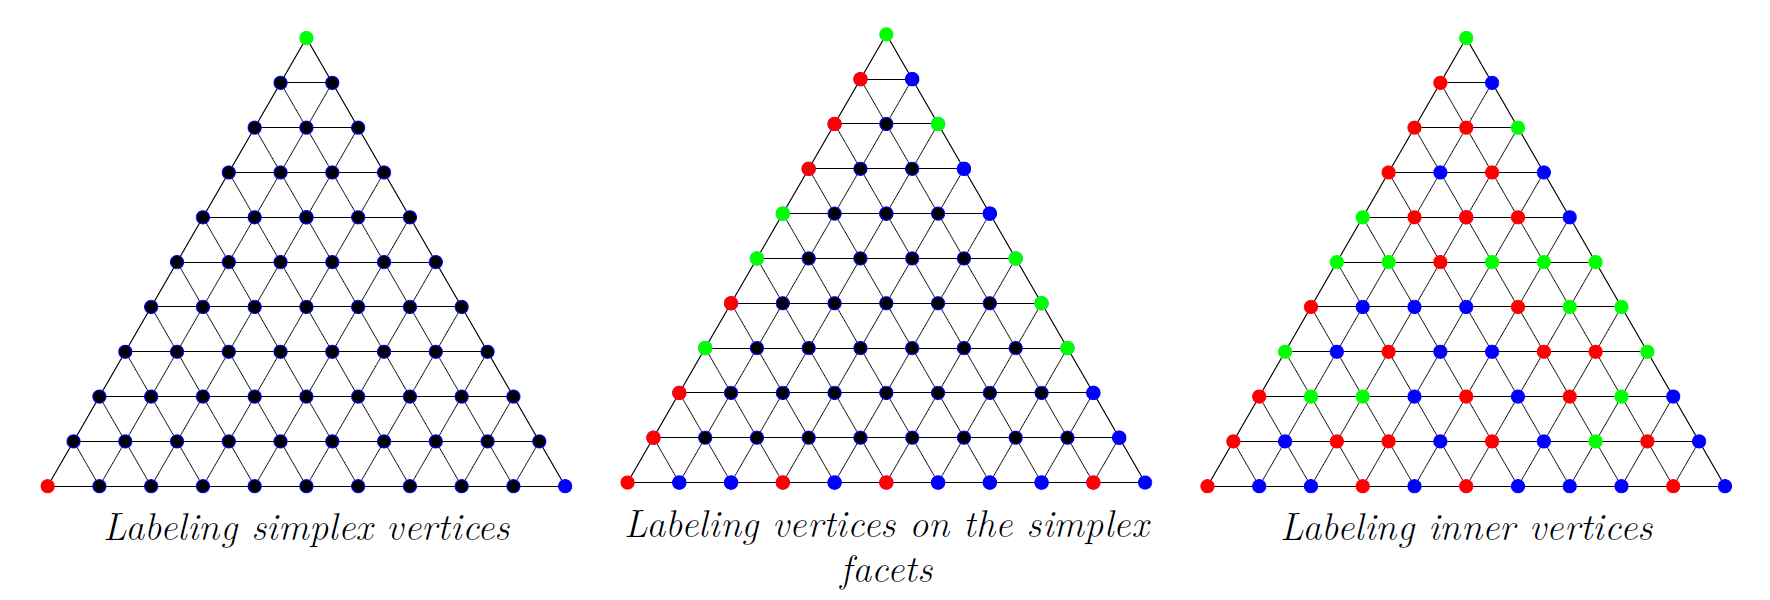
\includegraphics[width=\textwidth]{images/img_2_10_01.png}
\end{figure}
\noindent
\textbf{Exercise 10.0.2} (Panchromatic and quasi–panchromatic subsimplex). \textit{Provide the definitions of panchromatic and quasi–panchromatic n–dimension subsimplex.}\\\\
(Panchromatic (completely labeled) subsimplex). A subsimplex is called completely labeled or panchromatic if each vertex has a label different from the one of all the other vertices of the subsimplex. Therefore, a panchromatic n-dimensional subsimplex has $n+1$ different labels.\\\\
(Quasi-panchromatic (almost completely labeled) subsimplex). An n dimensional subsimplex is called almost completely labeled or quasi panchromatic if each vertex has a label different from the one of all the other vertices of the subsimplex except one. Therefore, a panchromatic n-dimensional subsimplex has n different labels among which one label is present twice.\\\\
\textbf{Exercise 10.0.3} (Sperner’s Lemma). \textit{Provide the statement of the Sperner’s Lemma.}\\\\
(Sperner’s Lemma). Given a n-dimensional simplex, a simplicial subdivion $ \mathcal{D} $, and a Sperner’s labeling $l$, there exists an odd number of panchromatic n-dimensional subsimplices. Therefore, there exists at least one panchromatic subsimplex.\\\\
\textbf{Exercise 10.0.4} (Sperner’s walk). \textit{Provide the definition of Spener’s walk and its characterization.}\\\\
(Sperner’s walk). Given a n-dimensional simplex $\Delta^n$, a simplicial subdivion $ \mathcal{D} $, and a Sperner’s labeling $l$, a Sperner’s walk is a sequence of adjacent subsimplices such that each common facet traversed to move from a subsimplex to the adjacent subsimplex has the same n different labels, that is $L \setminus \{s\}$ for some $s \in L$.
Therefore, each subsimplex of the walk is either quasi panchromatic or panchromatic.\\\\
(Sperner’s walk characterization). There are four main classes of Sperner’s walks:
\begin{itemize}
\item a sequence of subsimplices starting from a subsimplex with a facet on a facet of the simplex and ending in a subsimplex with a face on the same facet of the simplex without traversing any panchromatic subsimplex or any subsimplex with a facet on of the other facets of the simplex;
\item a sequence of subsimplices starting from a subsimplex with a facet on a facet of simplex and ending in a panchromatic subsimplex;
\item a cycle of subsimplices without any panchromatic subsimplex;
\item a sequence of subsimplices starting from a panchromatic subsimplex and ending in a panchromatic subsimplex.
\end{itemize}
Except walks strictly contained in the walks of the above four classes, no other Sperner’s walks are possible.\\\\
\textbf{Exercise 10.0.5} (Scarf’s algorithm). \textit{Describe the Scarf’s algorithm and its properties.}\\\\
(Scarf's algorithm). We describe the algorithm for the 2-dimensional case. Given a 2-dimensional simplex $\Delta^{2}$ and a simplicial subdivion $\mathcal{D},$ we embed $\Delta^{2}$ in a larger simplex $\bar{\Delta}^{2}$ as follows. Each vertex $v$ of $\bar{\Delta}^{2}$ is assigned a different label and it is connected to all the vertices of the subsimplices of $\Delta^{2}$ of a given facet such that one of the two labels appearing in the facet is the label of $v$. Two different vertices $v, v^{\prime}$ of $\bar{\Delta}^{2}$ are connected to the vertices of different facets of $\bar{\Delta}^{2}$ except for the vertices of the simplex $\Delta^{2}$ that belong to different facets. Furthermore, the three vertices of $\bar{\Delta}^{2}$ are connected with each other. Thus, there is a fictitious simplex composed of the whole space outer than $\bar{\Delta}^{2}$ that is panchromatic. This simplex is the starting point of the Scarf's algorithm.\\
The algorithm follows a Sperner's walk leaving this simplex (notice that three different paths can follow). Each path will end in a panchromatic subsimplex.\\
We report below the construction needed for the application of the Scarf’s algorithm and a path generated by an execution of the algorithm, specifically when the first traversed segment has colors blue and green.
\begin{figure}[H]
\centering
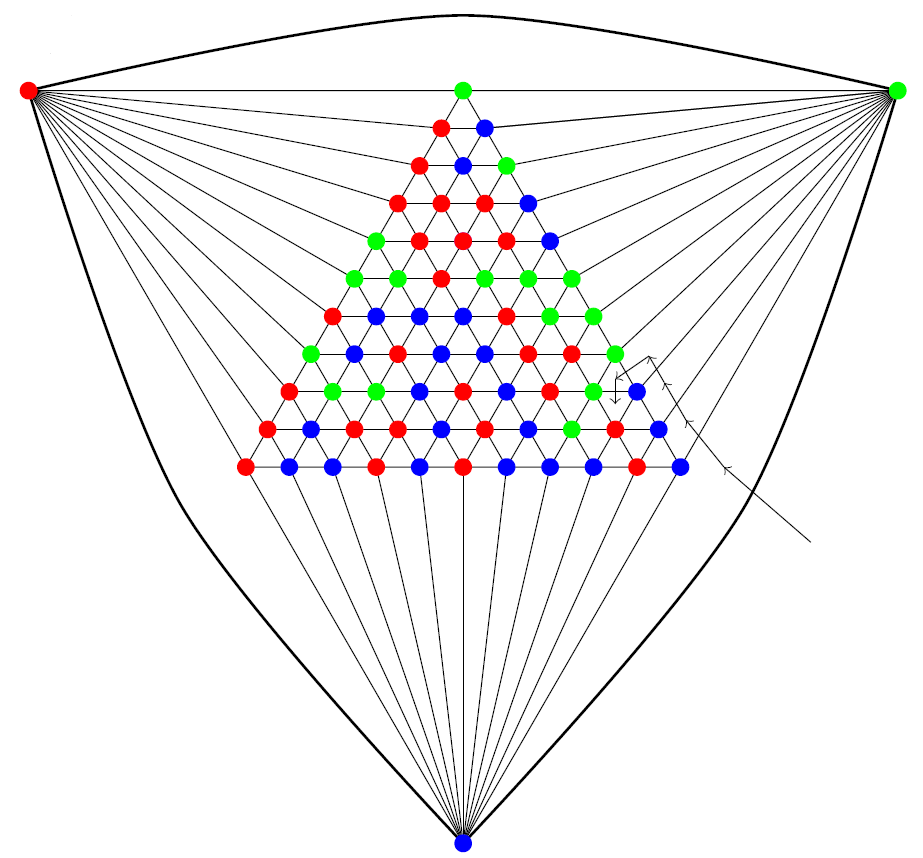
\includegraphics[width=\textwidth]{images/img_2_10_02.png}
\end{figure}
\noindent
\textbf{Exercise 10.0.6} (Solving 2–dimension Sperner). \textit{Given a 2–dimension simplex with a simplicial subdivision and a Sperner’s labeling, find a panchromatic subsimplex by means of Scarf’s algorithm (three examples of exercises follow). Do that for all three possible initializations of the Scarf’s algorithm.}\\\\
Credo...
\begin{figure}[H]
\centering
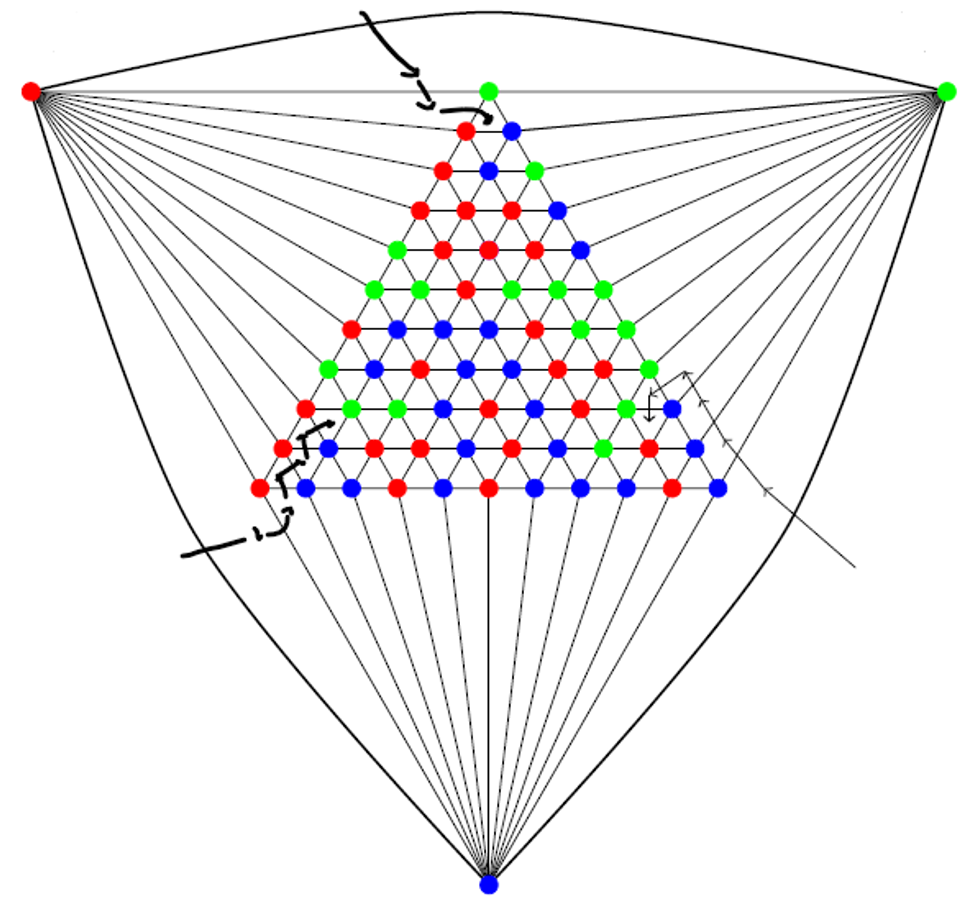
\includegraphics[width=\textwidth]{images/img_2_10_03.png}
\end{figure}
\noindent
\section{EC 2.11}

\textbf{Exercise 1} (END–OF–LINE). \textit{Provide the definition of the END–OF–LINE problem.}\\\\
(END-OF-LINE problem). END-OF-LINE is a problem characterized as follows:
\begin{itemize}
\item a graph composed of a potentially exponential number $O(2^n)$ of vertices labeled by a sequence of n bits;
\item a function $s : \{0, 1\}^n \rightarrow \{0, 1\} \cup \{N\}$ polynomially computable that, given a vertex, returns the unique
successor, if this exists, and N otherwise;
\item a function $p : \{0, 1\}^n \rightarrow \{0, 1\} \cup \{N\}$ polynomially computable that, given a vertex, returns the unique successor, if this exists, and N otherwise;
\item a node without predecessor;
\item the question is the finding of a leaf vertex (i.e., a vertex without either a predecessor or a successor).
\end{itemize}
\textbf{Exercise 2} (PPAD class). \textit{Provide the definition of PPAD computational class and its relationship with TFNP, FNP, and FNP–completeness.}\\\\
(\textsf{PPAD} complexity class). The \textsf{PPAD} complexity class is composed of all the problems P such that there is a polynomial-time reduction from P to \textsf{END-OF-LINE} problem, i.e., each instance of \textsf{P} can be formulated as an instance of \textsf{END-OF-LINE} whose size is bounded by a polynomial in the size of P.\\
In other words, a searching problem is in \textsf{PPAD} whether it can be solved by means of a path-following algorithm that starts from a source and, following a path, achieves a sink corresponding to a solution of the problem itself. We focus on the problems that are the hardest ones in the \textsf{PPAD} class.\\\\
(\textsf{PPAD} completeness). The set of \textsf{PPAD}-complete problems is a subset of \textsf{PPAD} problems containing all the problems P such that there is a polynomial-time reduction from END-OF-LINE to P.\\
Easily, a problem is \textsf{PPAD}-complete when it can be reduced from the \textsf{END-OF-LINE} problem. Furthermore, it is commonly believed the following.\\\\
(\textsf{PPAD} completeness and \textsf{FP}). It is commonly conjectured that the class of \textsf{PPAD}-complete problems is not in \textsf{FP}.\\
Therefore, the common conjecture is that $\mathsf{FP} \subset \mathsf{PPAD} \subset \mathsf{FNP}$. A number of fixed-point problems are \textsf{PPAD} complete. We cite a few of these problems.\\
Manca relazione con TFNP e FNP-completeness.\\\\
\textbf{Exercise 3} (Nash complexity). \textit{Describe the computational complexity of finding a Nash equilibrium.}\\\\
(\textsf{PPAD}-completeness of Nash equilibrium finding in 2-player games). Finding a Nash equilibrium in 2-player games is \textsf{PPAD} complete.\\
(\textsf{PPAD} completeness of $\epsilon$-Nash equilibrium finding in games with 3 or more players). Finding an $\epsilon$-Nash equilibrium in games with 3 or more players is \textsf{PPAD} complete.\\
(Pure-strategy Nash equilibrium complexity). Once n is fixed, computing a pure-strategy Nash equilibrium is in \textsf{P} class.\\\\
\textbf{Exercise 4} (Sperner complexity). \textit{Describe the computational complexity of finding a panchromatic subsimplex in k–dimension Sperner’s problem.}\\\\
(k-dimensional Sperner’s Lemma \textsf{PPAD} completeness). Given $k \geqslant 2$, the problem of finding a panchromatic subsimplex of Sperner’s Lemma is \textsf{PPAD} complete.\\
This leads us to the following observation. That is, in the worst case, the Scarf’s algorithm is the best algorithm to find a panchromatic subsimplex.\\
(Scarf’s algorithm and Sperner’s Lemma complexity). No algorithm more efficient than the Scarf’s algorithm exists to find a panchromatic subsimplex of the Sperner’s Lemma unless $\mathsf{FP} = \mathsf{PPAD}$.

\section{EC 2.12}

\textbf{Exercise 12.0.1} (Nash equilibrium). \textit{Provide the definition of Nash equilibrium.}\\\\
(Nash equilibrium finding). The problem of finding a Nash equilibrium can be formulated as a mathematical programming problem
\begin{figure}[H]
\centering
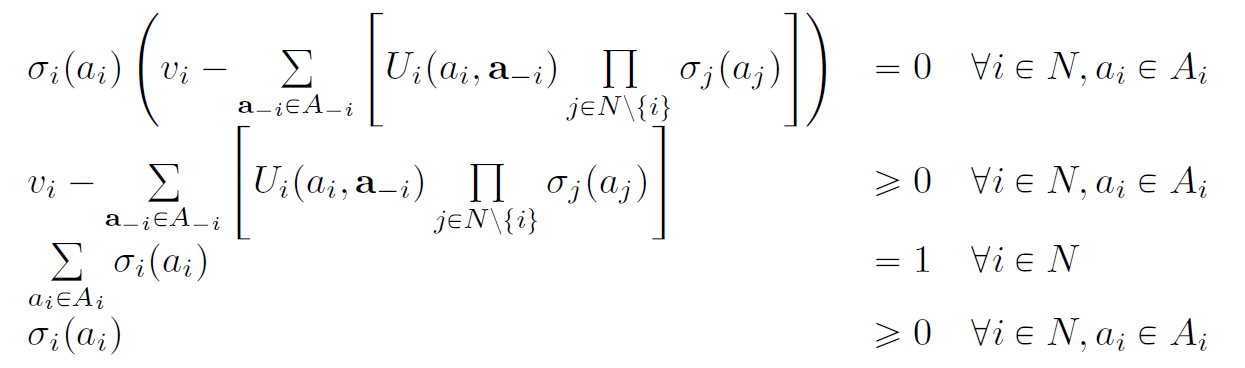
\includegraphics[width=\textwidth]{images/img_2_12_01.png}
\end{figure}
\noindent
whose nature is Non-Linear Complementarity Constraint (NLCP).\\
In the special case of 2 players, we have that the program reduced to a Linear Complementarity Program (LCP) as follows.\\\\
(Nash equilibrium finding with 2 players (LCP)). The problem of finding a Nash equilibrium with 2 players can be formulated as a mathematical programming problem
\begin{figure}[H]
\centering
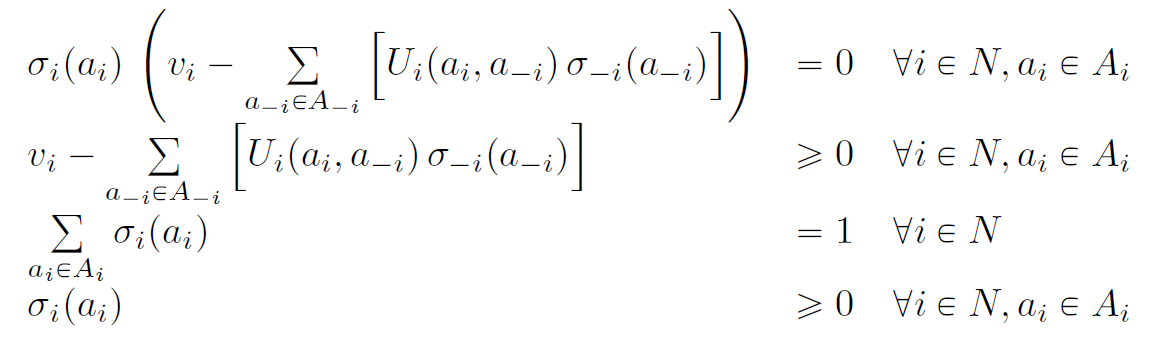
\includegraphics[width=\textwidth]{images/img_2_12_02.png}
\end{figure}
\noindent
whose nature is Linear Complementarity (LCP).\\
Let us remark that the program keeps to be nonlinear, variables $v_i and \sigma_i$ being multiplied together. However, an LCP have better properties than a generic NLCP. In particular, the solutions of an LCP have rational values, while the solution sof NLCP may have irrational values.\\\\
\textbf{Exercise 12.0.2} (Nash equilibrium example). \textit{Given a 2–player normal–form game with 2 actions per player, find all the Nash equilibria.}\\\\
\textcolor{red}{TODO}\\\\
\textbf{Exercise 12.0.3} (Mathematical programming formulation for normal–form games). \textit{Given an 2–player normal–form game, provide the MILP/MINLP program for finding a Nash equilibrium and show its derivation.}\\\\
(Nash equilibrium finding with 2 players (MILP)). The problem of finding a Nash equilibrium with 2 players can be formulated as a mathematical programming problem
\begin{figure}[H]
\centering
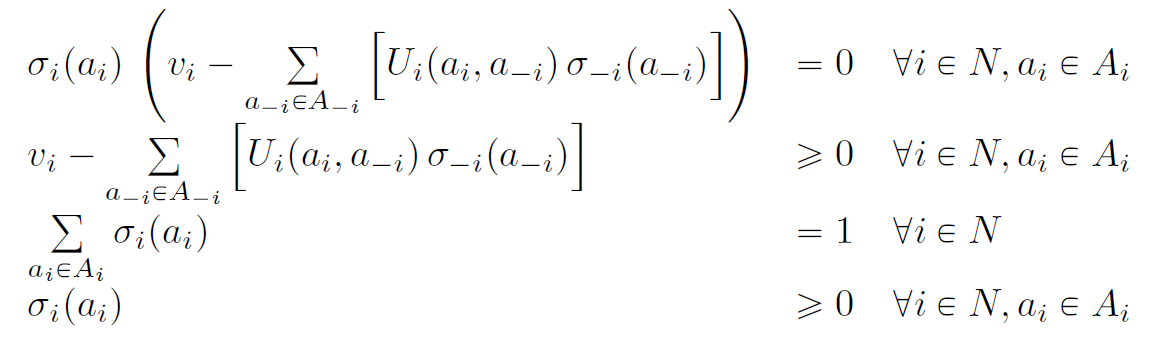
\includegraphics[width=\textwidth]{images/img_2_12_02.png}
\end{figure}
\noindent
whose nature is Mixed-Integer Linear (MILP); the constant $M_i$ can be set as $M_i = \max_{a}\{U_i (\mathbf{a})\} - \min_{a}\{U_i (\mathbf{a})\}$\\\\
\textit{Proof.} We just need to show that this reformulation is equivalent to the previous LCP one. The novelty resides in the adoption of binary variables $b_{i}$. The rationale is that an action $a_{i}$ can be played with strictly positive probability only if $b_{i}\left(a_{i}\right)$ is equal to $1 .$ This latter condition holds only the expected utility given by playing action $a_{i}$ equals $v_{i}$. Indeed, if $b_{i}\left(a_{i}\right)=1,$ we have that the term $M_{i}\left(1-b_{i}\left(a_{i}\right)\right)=0$ and therefore
$v_{i}=\sum_{a_{-i} \in A_{-i}}\left[U_{i}\left(a_{i}, a_{-i}\right) \sigma_{-i}\left(a_{-i}\right)\right]$. If instead $b_{i}\left(a_{i}\right)=0$, the expected utility given by action $a_{i}$ may be strictly
smaller than $v_{i},$ since we that $v_{i}-\sum_{a_{-i} \in A_{-i}}\left[U_{i}\left(a_{i}, a_{-i}\right) \sigma_{-i}\left(a_{-i}\right)\right] \leqslant M_{i}$ that is always true by construction of
$M_{i} .$ In other words, the adoption of a binary $b_{i}\left(a_{i}\right)$ allows one to enable or disable a set of constraints.\\\\
\textbf{Exercise 12.0.4} (Solving a normal–form game). \textit{Given a normal–form game with 2 players, find a Nash equilibrium by means of AMPL + GUROBI.}\\\\
\textcolor{red}{TODO}\\\\

\section{EC 2.13}

\textbf{Exercise 13.0.1} (Lemke–Howson’s labeling). \textit{Provide the definition of the Lemke–Howson’s labeling.}\\\\
The Lemke-Howson algorithm is a path-following algorithm working in 2-player normal-form games, returning an exact Nash equilibrium. Differently from the Scarf’s algorithm, the Lemke-Howson does not discretize the simplex space. Nevertheless, the Lemke-Howson algorithm is a combinatorial algorithm moving over a finite set
of points. Initially, we introduce the set of labels.\\\\
(Labels). The set of labels $L$ is defined as $L = \bigcup_{i \in N}{A_i}$. That is, we have one label for each action of each player.\\
(Solution labeling). A solution labeling $l$ is a function $l: \times_{i \in N} \Delta (A_i) \rightarrow \wp (L)$.
(Lemke-Howson's labeling). The Lemke-Howson's labeling $l$ is defined as follows:
$$
a_{i} \in l(\bm{\sigma}) \Longleftrightarrow\left(\left(\sigma_{i}\left(a_{i}\right)=0\right) \vee\left(v_{i}=\sum_{a_{-i} \in A_{-i}} U_{i}\left(a_{i}, a_{-i}\right) \sigma_{-i}\left(a_{-i}\right)\right)\right)
$$
\textbf{Exercise 13.0.2} (Lemke–Howson’s algorithm definition). \textit{Provide the sketch of the Lemke–Howson’s algorithm.}\\\\
(Lemke-Howson (rationale)). The algorithm is structured as follows.
\begin{itemize}
\item Partition the simplex of player $i$ in terms of best response of player $-i$. Each strategy profile $\mathbf{\sigma}$ corresponds
to a pair of points, one in the simplex of player 1 and one in the simplex of player 2. Each strategy profile $\mathbf{\sigma}$ is associated with a number of labels according to the Lemke-Howson labeling.
\item Focus on the nodes obtained by the intersections between the best response conditions and simplex border. Each node has three different labels (in degenerate games the labels may be more than three). The algorithm moves only between nodes.
\item Focus on completely labeled solutions and almost completely labeled solutions. An almost completely labeled solution $\mathbf{\sigma}$ presents a label, say \textsf{a}, twice. One is given in the simplex of player 1, while the other is given by the simplex of player 2. Therefore, given an almost completely labeled solution $\mathbf{\sigma}$, there are two ways to remove the label that appears twice: moving in the simplex of player 1 and moving in the
simplex of player 2. This means that moving along almost completely labeled solutions the algorithm moves along paths. These paths can be either cycles or non-cycles in which the starting solution and
the ending solution are completely labeled solutions.
\item Start from an artificial completely labeled solution: $\sigma_i (a_i) = 0$ for every $i \in N$ and for every $a_i \in A_i$.
And move along almost completely labeled solutions until find a completely labeled solution.
\end{itemize}
\textbf{Exercise 13.0.3} (Lemke–Howson’s algorithm application). \textit{Given a 2–player game with 3 actions per player and the partitioning of the simplices based on the opponent’s best responses, provide the labels associated with each area and apply the Lemke–Howson algorithm with three different initializations, corresponding to the three actions of player 1 (two examples of exercises follow).}\\\\
Consider the following 2-player game:
\begin{figure}[H]
\centering
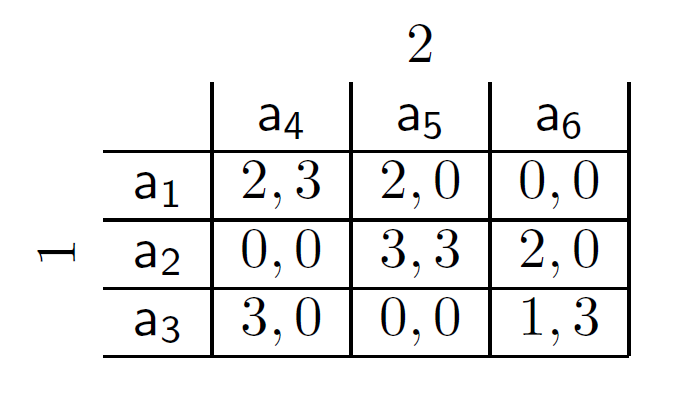
\includegraphics[width=0.4\textwidth]{images/img_2_13_01.png}
\end{figure}
\noindent
and the following strategy profile:
$$
\sigma_{1}\left(a_{1}\right)=\left\{\begin{array}{ll}
0.5 & \mathrm{a}_{1} \\
0.5 & \mathrm{a}_{2} \\
0.0 & \mathrm{a}_{3}
\end{array} \quad \sigma_{2}\left(a_{2}\right)=\left\{\begin{array}{ll}
0.5 & \mathrm{a}_{4} \\
0.0 & \mathrm{a}_{5} \\
0.5 & \mathrm{a}_{6}
\end{array}\right.\right.
$$
We have that $l( \mathbf{\sigma} ) = \{a_3, a_4, a_5\}$. Indeed, $a_3$ is the only best response of player 1 and therefore the labels of $a_1$ and $a_2$ that are played with strictly positive probability cannot be in $l( \mathbf{\sigma} )$, while both $a_4$ and $a_5$ are best response of player 2 and therefore the label of $a_6$ that is played with strictly positive probability cannot be in $l(\mathbf{\sigma})$.\\\\
(Lemke-Howson). Consider the following 2-player game:
\begin{figure}[H]
\centering
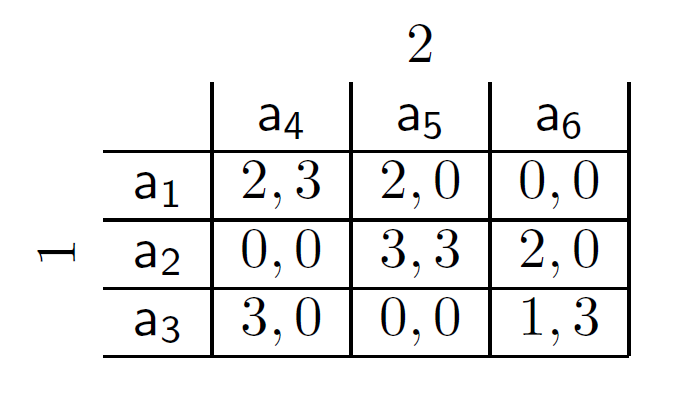
\includegraphics[width=0.4\textwidth]{images/img_2_13_01.png}
\end{figure}
\noindent
We report graphically the functioning of the algorithm.
\begin{figure}[H]
\centering
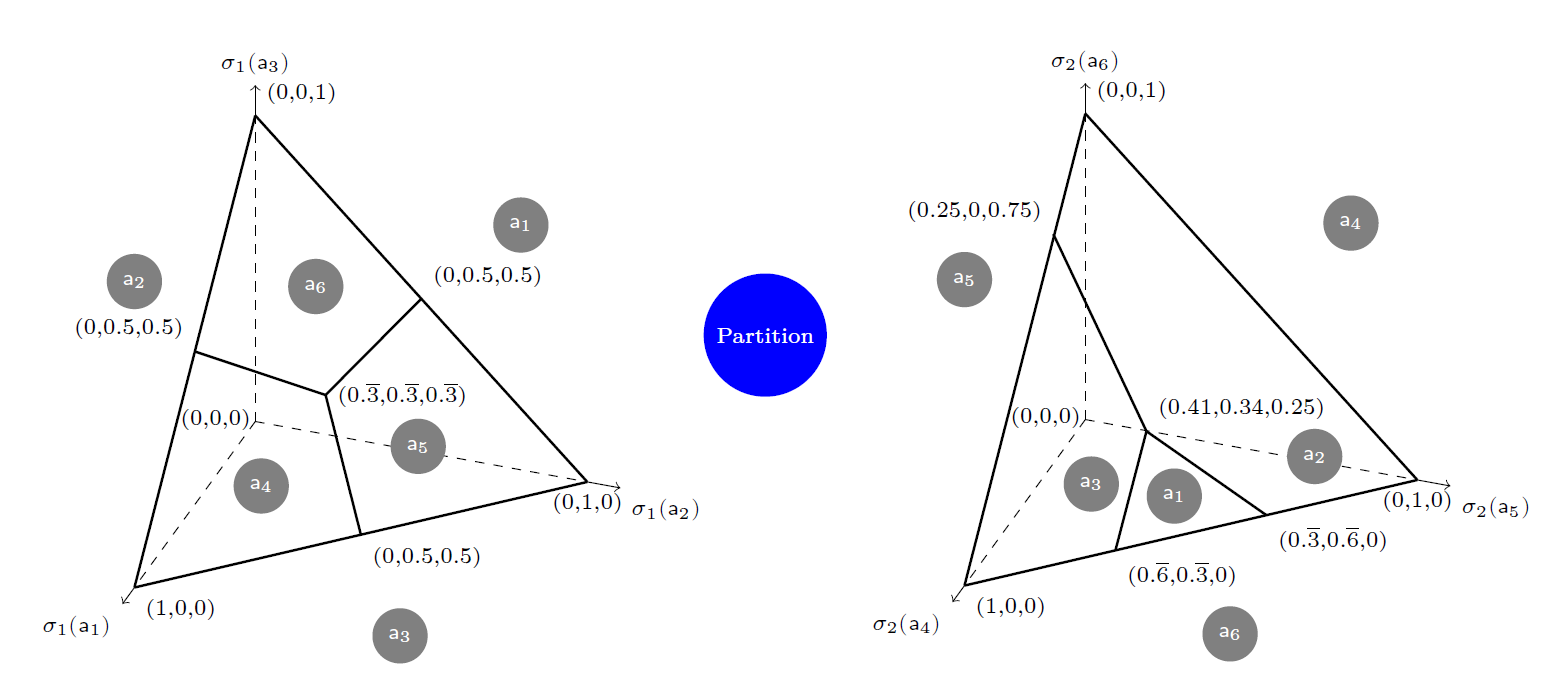
\includegraphics[width=\textwidth]{images/img_2_13_02.png}
\end{figure}
\begin{figure}[H]
\centering
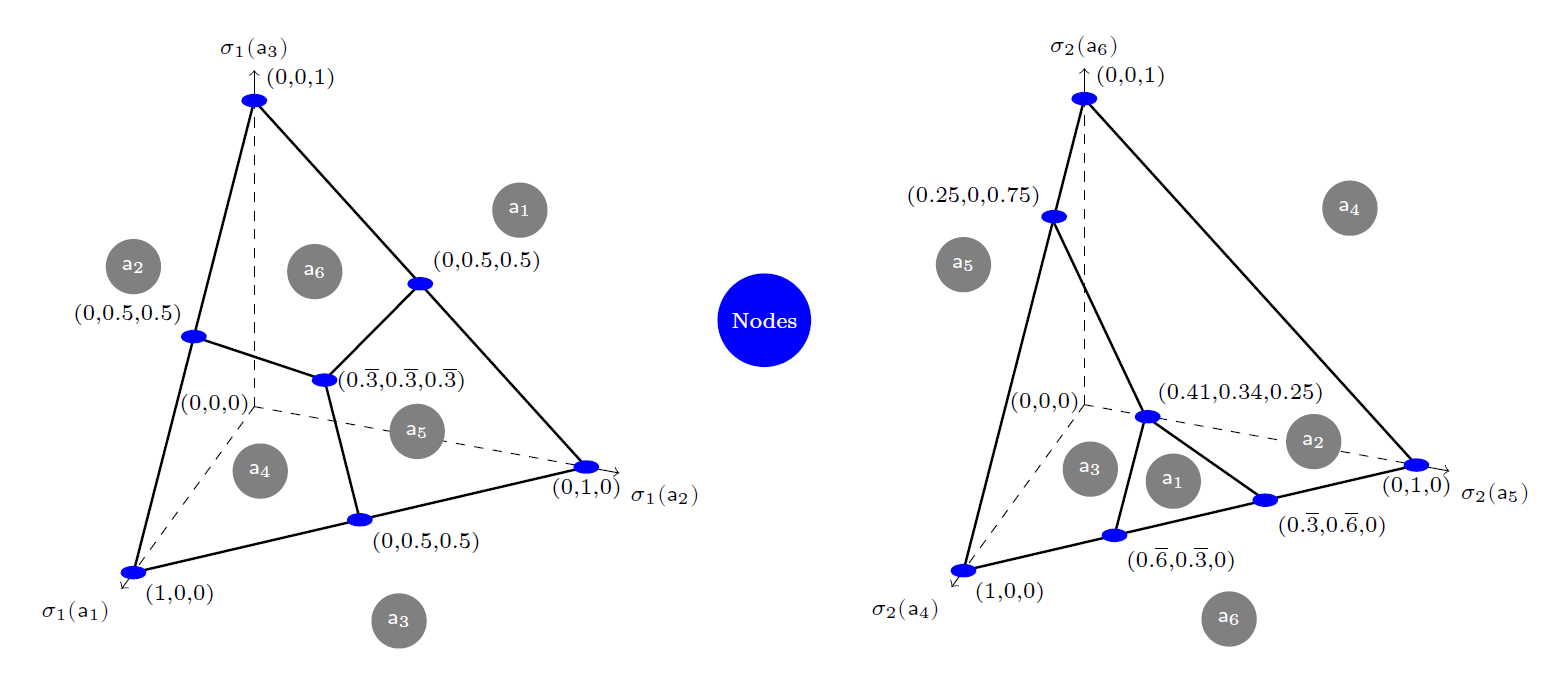
\includegraphics[width=\textwidth]{images/img_2_13_03.png}
\end{figure}
\begin{figure}[H]
\centering
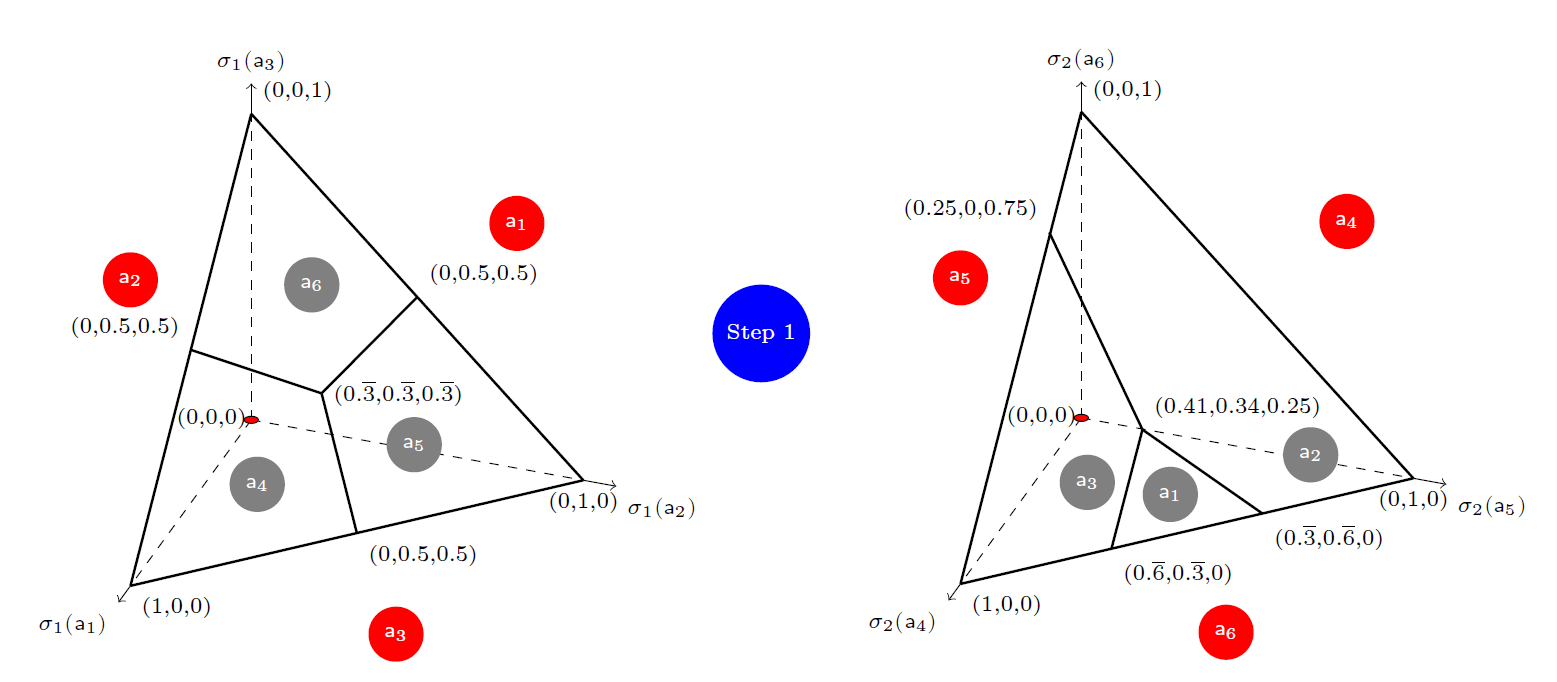
\includegraphics[width=\textwidth]{images/img_2_13_04.png}
\end{figure}
\begin{figure}[H]
\centering
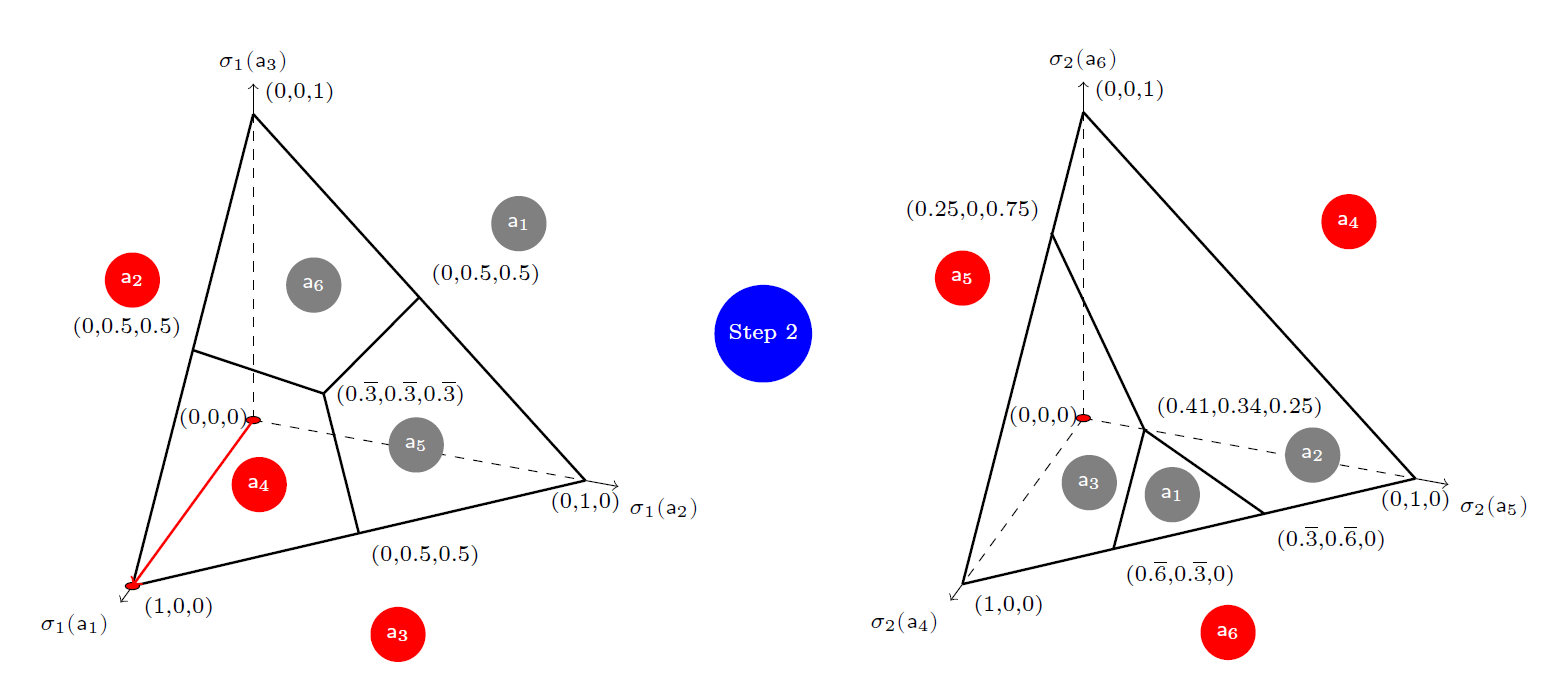
\includegraphics[width=\textwidth]{images/img_2_13_05.png}
\end{figure}
\begin{figure}[H]
\centering
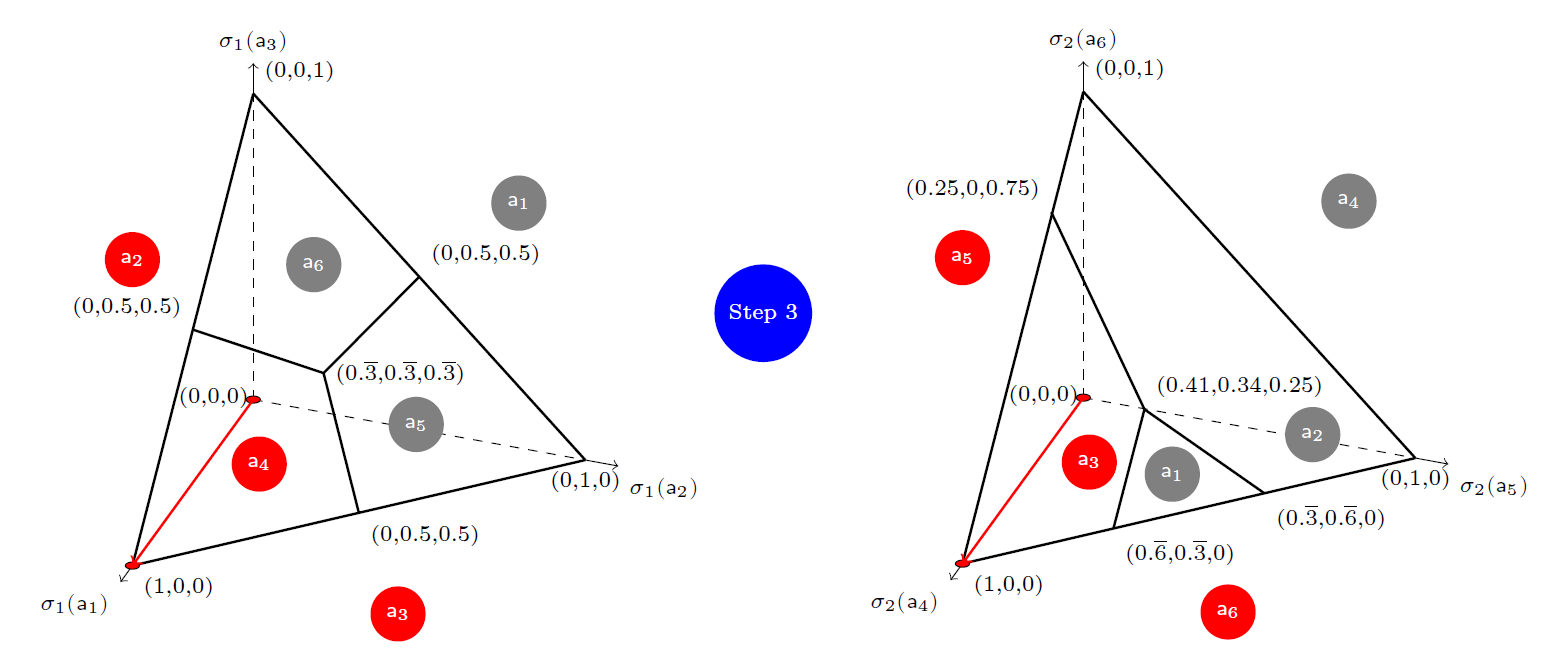
\includegraphics[width=\textwidth]{images/img_2_13_06.png}
\end{figure}
\begin{figure}[H]
\centering
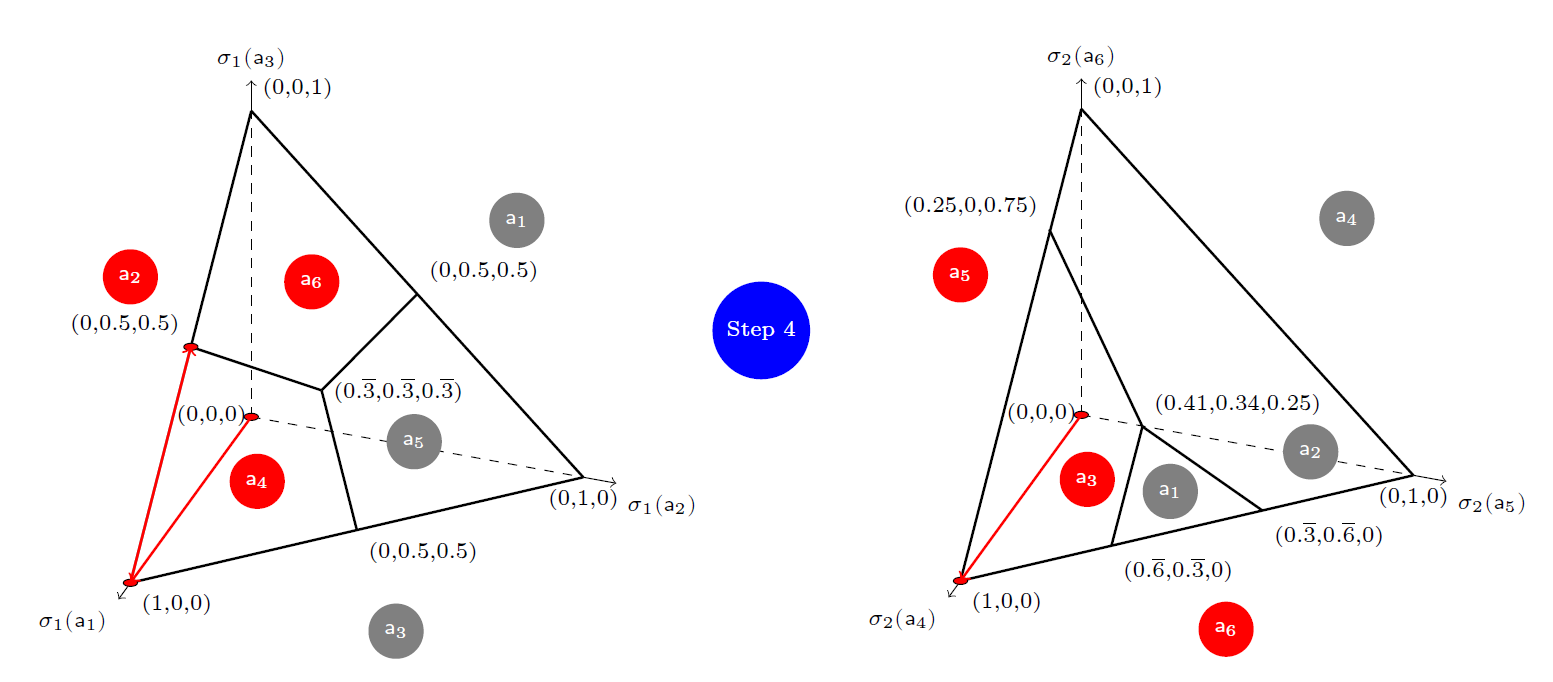
\includegraphics[width=\textwidth]{images/img_2_13_07.png}
\end{figure}
\begin{figure}[H]
\centering
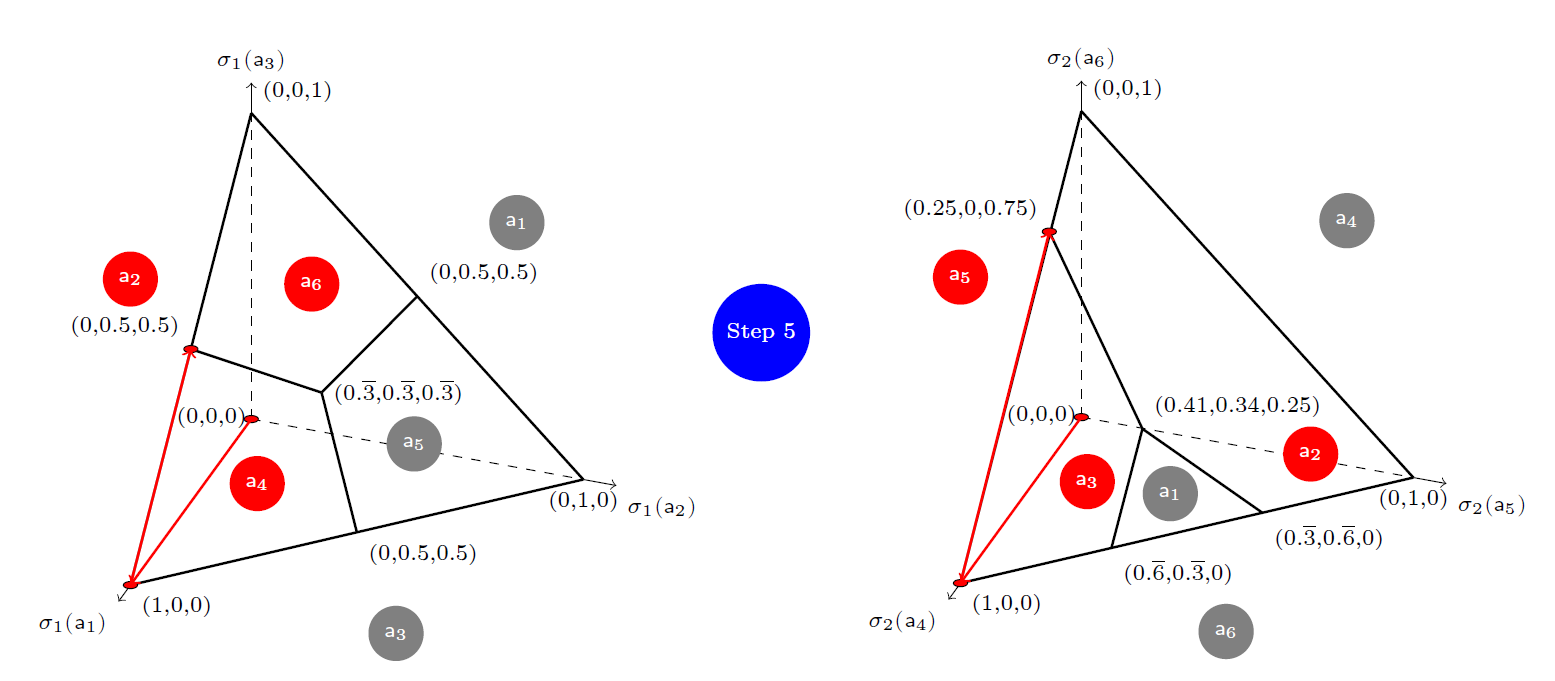
\includegraphics[width=\textwidth]{images/img_2_13_08.png}
\end{figure}
\begin{figure}[H]
\centering
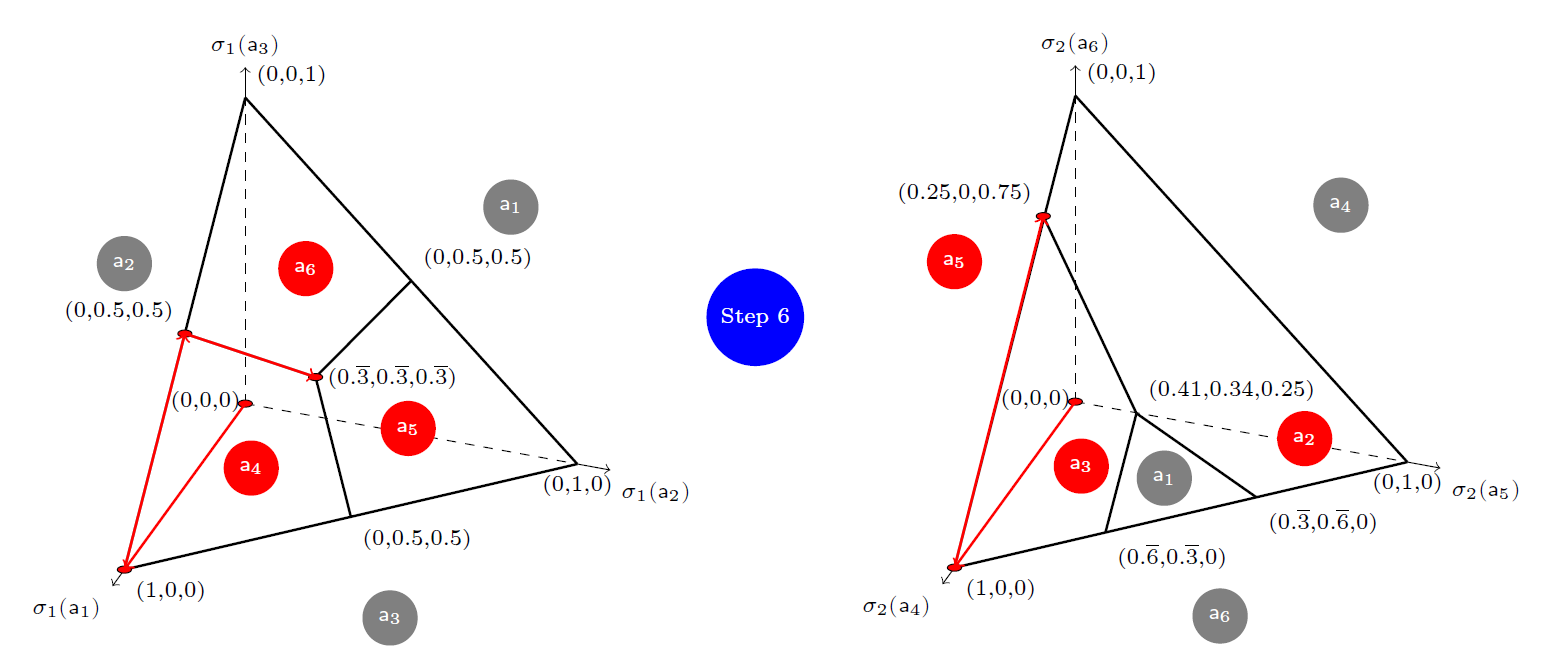
\includegraphics[width=\textwidth]{images/img_2_13_09.png}
\end{figure}
\begin{figure}[H]
\centering
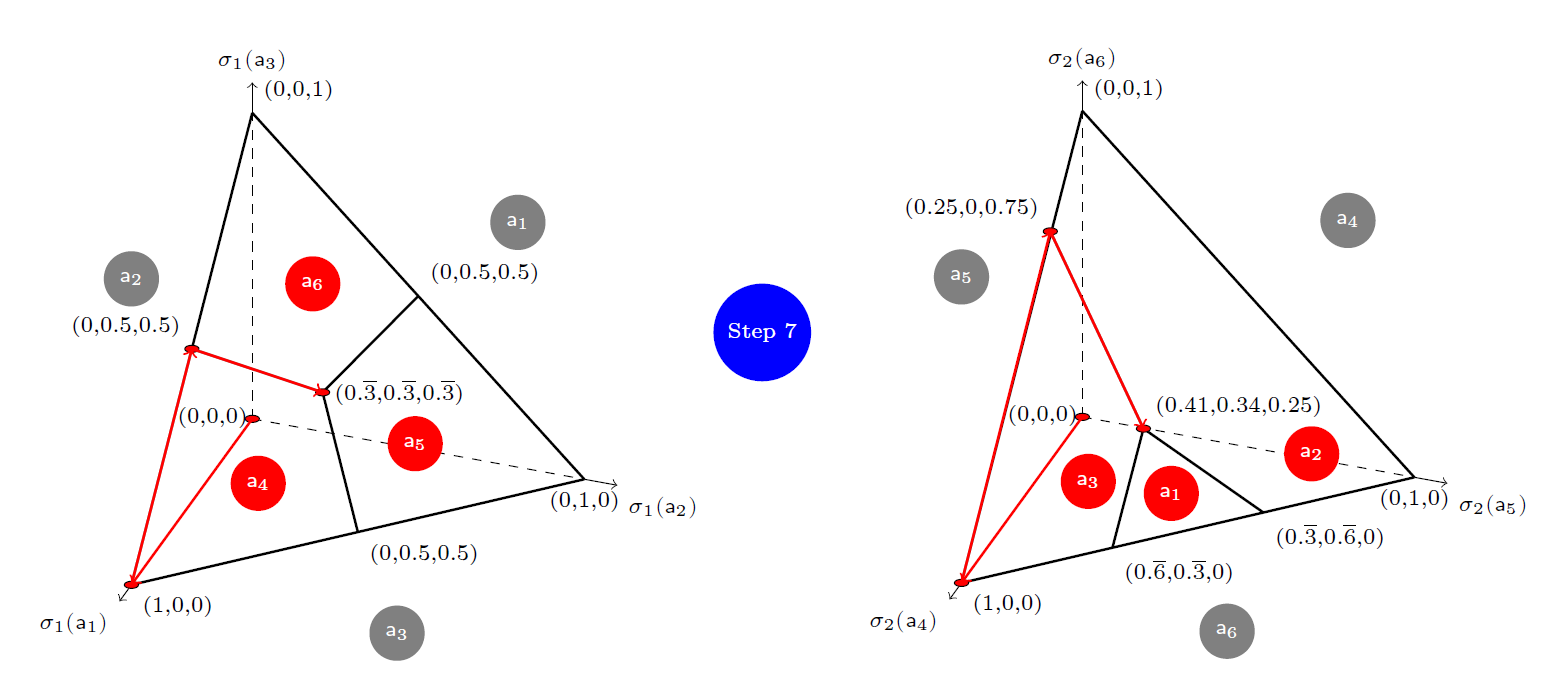
\includegraphics[width=\textwidth]{images/img_2_13_10.png}
\end{figure}